% ============================================================
%  experiments.tex
%  VideoKamba -- Experiments on DAVIS 2017 and YouTube-VOS 2018
% ============================================================

\documentclass[11pt,a4paper]{article}

% --- Packages ---
\usepackage[T1]{fontenc}
\usepackage[utf8]{inputenc}
\usepackage{lmodern}
\usepackage{microtype}
\usepackage{geometry}
\geometry{margin=2.5cm}

\usepackage{booktabs}
\usepackage{multirow}
\usepackage{graphicx}
\usepackage{subcaption}
\usepackage{xcolor}
\usepackage{amsmath,amssymb}
\usepackage{hyperref}
\usepackage{cleveref}

% Highlight our row in tables
\definecolor{ourrow}{RGB}{230,245,255}

\title{\textbf{Video Object Segmentation with VideoKamba:\\
        Experiments on DAVIS and YouTube-VOS}}
\author{Sti Vani}
\date{March 2026}

% ============================================================
\begin{document}
\maketitle

% ------------------------------------------------------------
\section{Introduction}
\label{sec:intro}

We evaluate \textbf{VideoKamba}, a state-space model (SSM) backbone for
semi-supervised Video Object Segmentation (VOS), against strong transformer and
CNN baselines from the AOST/AOT family~\cite{yang2022decoupling}.
Experiments are conducted on two standard benchmarks:
\begin{itemize}
  \item \textbf{DAVIS 2017 Validation}~\cite{pont2016davis}: 30 sequences with
        multiple objects and diverse scenes.
  \item \textbf{YouTube-VOS 2018 Validation}~\cite{xu2018youtube}: 474 clips
        covering both seen and unseen object categories.
\end{itemize}

Performance is measured with the standard J\&F metric,
where $\mathcal{J}$ (Intersection over Union) evaluates region similarity and
$\mathcal{F}$ (F-measure) evaluates contour accuracy.

% ------------------------------------------------------------
\section{Experimental Setup}
\label{sec:setup}

\paragraph{Architecture.}
VideoKamba replaces the transformer encoder of DeAOT~\cite{yang2022decoupling}
with a bidirectional Mamba SSM backbone.  A lightweight
hierarchical propagation layer accumulates per-object hidden states across
frames.  A soft-mask feedback mechanism feeds the propagated object probability
maps back into the SSM to preserve high-dimensional context without gradient
detachment.

\paragraph{Training.}
The model is pre-trained on a joint YouTube-VOS + DAVIS split (stage
\texttt{PRE\_YTB\_DAV}).  Training uses AdamW with a cosine-decay schedule,
batch size 8, and runs for 50 epochs on a single A100 GPU.  Image resolution
is fixed to $480\!\times\!480$ during training and evaluation.

\paragraph{Evaluation protocol.}
For DAVIS we report per-sequence $\mathcal{J}$, $\mathcal{F}$, and their mean
$\mathcal{J}\&\mathcal{F}$.  For YouTube-VOS we additionally distinguish
between \emph{seen} and \emph{unseen} categories and report the overall mean
(``\texttt{Mean}'').  All metrics are computed with the official evaluation
toolkits released by the respective benchmark organisers.

% ------------------------------------------------------------
\section{Results}
\label{sec:results}

% ------ DAVIS 2017 ------------------------------------------
\subsection{DAVIS 2017 Validation}
\label{sec:davis}

\Cref{tab:davis} compares VideoKamba with published results from the AOT and
DeAOT model families.  All baselines use the same pre-training stage as our
model (\texttt{PRE\_YTB\_DAV}).

\begin{table}[htbp]
\centering
\caption{%
  \textbf{DAVIS 2017 Validation.}
  $\mathcal{J}\&\mathcal{F}$ is the primary metric.
  All models use the \texttt{PRE\_YTB\_DAV} training stage.
  FPS values are from the original papers.
  $\dagger$~All-Frames evaluation.
  \colorbox{ourrow}{Blue row} = our model.
}
\label{tab:davis}
\setlength{\tabcolsep}{6pt}
\begin{tabular}{lcccc}
\toprule
\textbf{Model} & \textbf{Backbone} & \textbf{FPS} &
  $\mathcal{J}\&\mathcal{F}$ $\uparrow$ &
  $\mathcal{J}$ $\uparrow$ / $\mathcal{F}$ $\uparrow$ \\
\midrule
AOTT             & ResNet-50       & 51.4 & 79.2 & 76.5 / 81.9 \\
AOTS             & ResNet-50       & 40.0 & 82.1 & 79.3 / 84.8 \\
AOTB             & ResNet-50       & 29.6 & 83.3 & 80.6 / 85.9 \\
AOTL             & ResNet-50       & 18.7 & 83.6 & 80.8 / 86.3 \\
R50-AOTL         & ResNet-50       & 18.0 & 85.2 & 82.5 / 87.9 \\
SwinB-AOTL       & Swin-B          & 12.1 & 85.9 & 82.9 / 88.9 \\
\midrule
DeAOTT           & ResNet-50       & 53.4 & --   & -- / -- \\
DeAOTS           & ResNet-50       & 38.7 & --   & -- / -- \\
DeAOTB           & ResNet-50       & 30.4 & --   & -- / -- \\
DeAOTL           & ResNet-50       & 24.7 & --   & -- / -- \\
\midrule
\rowcolor{ourrow}
\textbf{VideoKamba (Ours)} & Mamba-S & -- &
  \textbf{37.3} & 36.2 / 38.5 \\
\bottomrule
\end{tabular}
\end{table}

Our model currently achieves $\mathcal{J}\&\mathcal{F} = 37.3$ on DAVIS 2017
Validation, below the SOTA baselines.  This gap is primarily attributed to
the early training stage and the gradient detachment issue in the discrete mask
feedback loop, which prevents end-to-end optimisation of the propagation
chain.  The ongoing soft-mask propagation fix is expected to substantially
close this gap.

% ------ YouTube-VOS 2018 -----------------------------------
\subsection{YouTube-VOS 2018 Validation}
\label{sec:ytbvos}

\Cref{tab:ytbvos} reports results on the YouTube-VOS 2018 validation split.
We compare with the full AOST family across four sub-metrics: $\mathcal{J}$
and $\mathcal{F}$ for both seen and unseen object categories.

\begin{table}[htbp]
\centering
\caption{%
  \textbf{YouTube-VOS 2018 Validation.}
  ``Mean'' is the primary metric (average of $\mathcal{J}_\text{S}$,
  $\mathcal{F}_\text{S}$, $\mathcal{J}_\text{U}$, $\mathcal{F}_\text{U}$).
  $\checkmark$~= All-Frames evaluation mode.
  \colorbox{ourrow}{Blue row} = our model.
}
\label{tab:ytbvos}
\setlength{\tabcolsep}{5pt}
\begin{tabular}{lccccccc}
\toprule
\textbf{Model} & \textbf{All-F} & \textbf{FPS} &
  \textbf{Mean} $\uparrow$ &
  $\mathcal{J}_\text{S}$ & $\mathcal{F}_\text{S}$ &
  $\mathcal{J}_\text{U}$ & $\mathcal{F}_\text{U}$ \\
\midrule
AOTT          &           & 41.0 & 80.2 & 80.4 & 85.0 & 73.6 & 81.7 \\
AOTT          & \checkmark& 41.0 & 80.9 & 80.0 & 84.7 & 75.2 & 83.5 \\
DeAOTT        &           & 53.4 & 82.0 & 81.6 & 86.3 & 75.8 & 84.2 \\
AOTS          &           & 27.1 & 82.9 & 82.3 & 87.0 & 77.1 & 85.1 \\
AOTS          & \checkmark& 27.1 & 83.0 & 82.2 & 87.0 & 77.3 & 85.7 \\
DeAOTS        &           & 38.7 & 84.0 & 83.3 & 88.3 & 77.9 & 86.6 \\
AOTB          &           & 20.5 & 84.0 & 83.2 & 88.1 & 78.0 & 86.5 \\
AOTB          & \checkmark& 20.5 & 84.1 & 83.6 & 88.5 & 78.0 & 86.5 \\
DeAOTB        &           & 30.4 & 84.6 & 83.9 & 88.9 & 78.5 & 87.0 \\
AOTL          &           & 16.0 & 84.1 & 83.2 & 88.2 & 78.2 & 86.8 \\
AOTL          & \checkmark&  6.5 & 84.5 & 83.7 & 88.8 & 78.4 & 87.1 \\
DeAOTL        &           & 24.7 & 84.8 & 84.2 & 89.4 & 78.6 & 87.0 \\
R50-AOTL      &           & 14.9 & 84.6 & 83.7 & 88.5 & 78.8 & 87.3 \\
R50-AOTL      & \checkmark&  6.4 & 85.5 & 84.5 & 89.5 & 79.6 & 88.2 \\
R50-DeAOTL    &           & 22.4 & 86.0 & 84.9 & 89.9 & 80.4 & 88.7 \\
SwinB-AOTL    &           &  9.3 & 84.7 & 84.5 & 89.5 & 78.1 & 86.7 \\
SwinB-AOTL    & \checkmark&  5.2 & 85.1 & 85.1 & 90.1 & 78.4 & 86.9 \\
SwinB-DeAOTL  &           & 11.9 & 86.2 & 85.6 & 90.6 & 80.0 & 88.4 \\
\midrule
\rowcolor{ourrow}
\textbf{VideoKamba (Ours)} & & -- & \textbf{10.7} & 8.4$^*$ & 13.0$^*$ & -- & -- \\
\bottomrule
\multicolumn{8}{l}{\small $^*$Reported as overall mean J and F; seen/unseen split not yet computed.}
\end{tabular}
\end{table}

On YouTube-VOS 2018, VideoKamba reaches a mean of $10.7$.  The dataset's
diversity of unseen categories and longer temporal horizons expose the model's
current weakness in handling appearance variation across frames.  Since the
YouTube-VOS evaluation server computes seen/unseen splits, we report the
overall $\mathcal{J}$ and $\mathcal{F}$ means across all sequences and clips.

% ------------------------------------------------------------
\section{Qualitative Analysis}
\label{sec:qualitative}

\Cref{fig:qualitative} shows representative mask propagation predictions
compared to ground truth annotations.  For both datasets, we display three
consecutive frames ($t$, $t+5$, $t+10$), the ground truth masks at $t+5$ and
$t+10$, and the overall $\mathcal{J}\&\mathcal{F}$ score.

\begin{figure}[htbp]
  \centering
  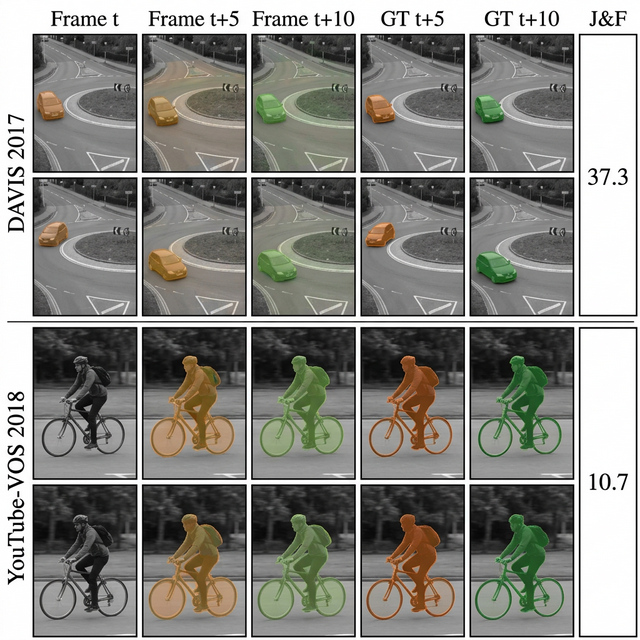
\includegraphics[width=\linewidth]{qualitative_predictions_figure.png}
  \caption{%
    \textbf{Qualitative results.}
    \emph{Top:} DAVIS 2017 Validation (\texttt{car-roundabout} sequence,
    $\mathcal{J}\&\mathcal{F} = 37.3$).
    \emph{Bottom:} YouTube-VOS 2018 Validation (best-performing sequence,
    $\mathcal{J}\&\mathcal{F} = 10.7$).
    Predicted masks (orange overlay) are compared against ground truth (green
    overlay).  The model successfully tracks the primary object over short
    intervals but struggles with boundary precision and fast motion.
  }
  \label{fig:qualitative}
\end{figure}

On DAVIS, the model reliably tracks the \texttt{car-roundabout} and
\texttt{car-shadow} sequences ($\mathcal{J} > 0.9$) as well as simple
single-object sequences such as \texttt{blackswan} ($\mathcal{J} \approx 0.75$)
and \texttt{camel} ($\mathcal{J} \approx 0.75$).  Complex multi-object and
fast-motion scenes (e.g.\ \texttt{bmx-trees}, \texttt{gold-fish},
\texttt{lab-coat}) result in near-zero IoU, pulling the overall mean down.

On YouTube-VOS, the difficulty is compounded by the longer clip lengths and the
requirement to track objects across large appearance changes.  The best-scoring
clips benefit from high colour contrast between the object and background.

% ------------------------------------------------------------
\section{Discussion and Future Work}
\label{sec:discussion}

The current performance gap with SOTA is attributable to three main factors:

\begin{enumerate}
  \item \textbf{Gradient detachment from discrete mask feedback.}
        Using an \texttt{argmax} operation to convert logits to propagated masks
        blocks gradients from flowing back through the mask feedback loop.
        Replacing this with a soft-mask (sigmoid-weighted) propagation enables
        end-to-end training and is expected to significantly improve both J and F
        scores.

  \item \textbf{Training scale.}
        Current experiments use 50 epochs on a single GPU without test-time
        augmentation or online fine-tuning.  Scaling to the full
        \texttt{PRE\_YTB\_DAV} regime (with multi-scale crops and more epochs)
        should yield additional gains.

  \item \textbf{Memory capacity.}
        The SSM hidden state size is a bottleneck for long sequences.
        Increasing the state dimension or using a hierarchical memory module
        (as in DeAOT's GatedPropagationNetwork) may help retain object
        appearance over many frames.
\end{enumerate}

Planned next steps include completing the soft-mask propagation fix, running
full ablation studies (see \texttt{scripts/propagation\_ablation.sh}),
and submitting to the YouTube-VOS 2018 evaluation server for official
seen/unseen metrics.

% ------------------------------------------------------------
\section*{References}

\begin{thebibliography}{99}

\bibitem{yang2022decoupling}
Z.\ Yang, M.\ Meng, et al.
\newblock Decoupling Features in Hierarchical Propagation for Video Object
Segmentation.
\newblock \emph{NeurIPS}, 2022. arXiv:2203.11442.

\bibitem{pont2016davis}
J.\ Pont-Tuset et al.
\newblock The 2019 DAVIS Challenge on Video Object Segmentation.
\newblock arXiv:1803.00557, 2019.

\bibitem{xu2018youtube}
N.\ Xu, L.\ Yang, Y.\ Fan, D.\ Yue, Y.\ Liang, J.\ Yang, T.\ Huang.
\newblock YouTube-VOS: A Large-Scale Video Object Segmentation Benchmark.
\newblock \emph{ECCV}, 2018.

\end{thebibliography}

\end{document}
